\chapter{Letra y ritmo musical}
\label{cap:letra-ritmo}

\begin{figure}[H]
\centering
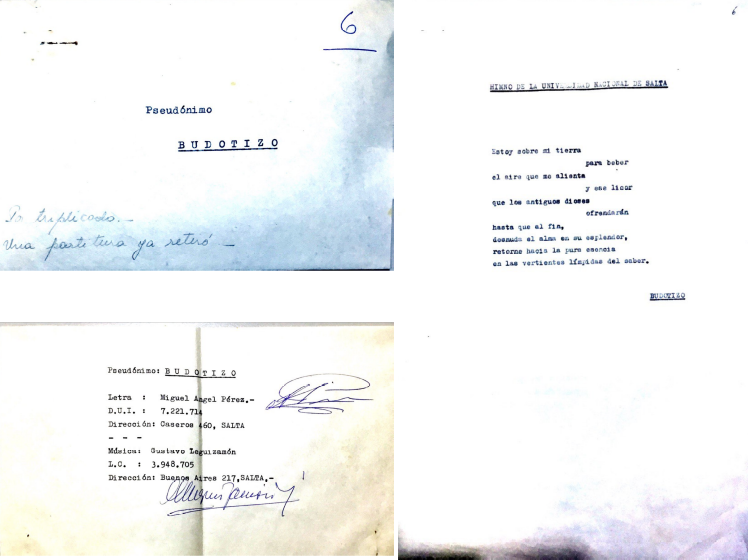
\includegraphics[width=0.6\textwidth]{img/sobre-seudonimo-poema}
\caption{Sobre, datos del seudónimo y letra del Himno.}
\label{fig:sobre-letra}
\end{figure}

\section{Himno a la Universidad Nacional de Salta}
\label{sec:himno-letra}

\texttt{ %\footnotesize
\begin{verse}
Estoy sobre mi tierra\\
\hspace{4cm}para beber\\
el aire que me alienta\\
\hspace{4cm}y ese licor\\
que los antiguos dioses\\
\hspace{4cm}ofrendarán\\
hasta que al fin,\\
desnuda el alma en su esplendor,\\
retorne hacia la pura esencia\\
en las vertientes límpidas del saber.
\end{verse}
\hspace{5cm} Miguel Ángel Pérez (1982)
}

\vspace{0.5cm}

En el Cuadro~\ref{tab:analisis-letra} (página~\pageref{tab:analisis-letra}) realizamos un breve análisis de la métrica del poema. En él notamos, como datos sobresalientes, que Leguizamón eligió \emph{siempre} utilizar las sinalefas, e incluso eligió unir con una sinalefa los dos últimos versos, de nueve y once sílabas cada uno, quedando como consecuencia diecinueve sílabas entre los dos versos.

\begin{table}[ht]
\centering
\rotatebox{90}
{
\begin{tabular}{@{}llll@{}}
\toprule
\multirow{2}{*}{Versos}                & \multicolumn{3}{c}{Sílabas}                  \\
                                       & sin sinalefas & con sinalefas & en la música \\
\midrule
Estoy sobre mi tierra {[} para beber   & 11            & 11            & 11           \\
el aire que me alienta {[} y ese licor & 13            & 11            & 11           \\
que los antiguos dioses {[} ofrendarán & 11            & 11            & 11           \\
hasta que al fin,                      & 5             & 4             & 4            \\
desnuda el alma en su esplendor,       & 11            & 8             & 8            \\
retorne hasta la pura esencia          & 11            & 9             & 9            \\
en las vertientes límpidas del saber.  & 11            & 11            & 11 (10)\tablefootnote{Los dos últimos versos soportan, al unirlos, una sinalefa entre ellos, que es usada por Leguizamón, haciendo así de los dos últimos un verso de diecinueve sílabas.}      \\
\bottomrule
\end{tabular}
}
\caption{Análisis silábico del poema de Miguel Ángel Pérez.}
\label{tab:analisis-letra}
\end{table}

\begin{table}[H]
\begin{minipage}{\textwidth}
\centering
\begin{tabular}{@{}ll@{}}
\toprule
ritmo-melodía-verso     & sílabas\footnote{Entre paréntesis anotamos las sílabas tal como se tienen en cuenta desde el pensamiento estrictamente literario, el cual contempla una sílaba más para versos terminados en acentuación aguda, mas nos quedamos con los números que coinciden con la cantidad de notas en el ritmo de la melodía.} \\
\midrule
\lilyfile{part/verso1}  & 11(12)  \\
\lilyfile{part/verso2}  & 11(12)  \\
\lilyfile{part/verso3}  & 11(12)  \\
\lilyfile{part/verso4}  & 4(5)    \\
\lilyfile{part/verso5}  & 8(9)    \\
\lilyfile{part/verso6}  & 19(20)  \\
\bottomrule
\end{tabular}
\end{minipage}
\caption[Resolución rítmico-melódica de la letra en la música.]{Resolución rítmico-melódica de la letra en la música.}
\label{tab:ritmo-letra}
\end{table}

El Cuadro~\ref{tab:ritmo-letra} aclara especialmente la resolución rítmico-melódica de los últimos cuatro versos de la letra, respetando en su unicidad el único verso de cuantro sílabas que posee el poema y, a continuación generando con los tres versos siguientes dos frases musicales de ocho y diecinueve sílabas respectivamente que proveen al final de la pieza de una asimetría que atenta contra el aburrimiento.

\begin{figure}[H]
\centering
\ritmo{\time 2/4 \partial 8 f8 f4. f8 f f f f f4 f8 f f4.}
\caption{Patrón rínmico predominante.}
\label{fig:patron-ritmico}
\end{figure}

El ritmo de la Figura~\ref{fig:patron-ritmico} es el patrón que marca todos los versos de once sílabas. La decisión compositiva de no continuar en los últimos tres versos con la métrica presente en el poema es fundamental a la hora de definir la estética de la pieza, ya que sin la ruptura de la simetría el sopor podría haberse adue;ado del final de esta canción.

Volviendo sobre el ritmo predominante en la pieza (Figura~\ref{fig:patron-ritmico}) esta vez en relación con la letra, debemos decir que en dos ocasiones sucede algo que es bastante habitual encontrar en la música popular: palabras acentuadas de manera diferente en la música a como son en el habla. La primera de éstas acontece entre los compases 1 y 2 \ritmoletra{\time 2/4 \partial 8 f8 f4. f8\upbow f\downbow f f f} {Es -- toy so -- bre la tie -- rra...}\footnote{Los símbolos \lilyGlyph{scripts.upbow} (punta) y \lilyGlyph{scripts.downbow} (talón) provienen de los conceptos de \emph{arsis} y \emph{thesis}, alzar y dar, al aire y a tierra, no acentuado y acentuado. El movimiento de un pie al caminar tiene esos dos momentos: no acentuado cuando se apoya sobre su punta, y acentuado cuando se apoya, en un nuevo paso, el talón. Los instrumentos de cuerda frotada heredan estos símbolos resignificándolos como punta y taco del arco e indican con qué parte del arco debe atacarse la nota señalada.} donde con la palabra \emph{sobre}, y la segunda, de forma análoga, sucede entre los compases 33 y 34 \ritmoletra{\time 2/4 \partial 8 f8 f4. f8\upbow f\downbow f f f} {re -- tor -- ne~ha -- cia la pu -- ra~e...} donde con la palabra \emph{hacia}, son acentuadas en forma aguda, siendo ellas, claramente, palabras de acentuación grave. Un tercer caso de cambio de acentuación se encuentra entre los compases 29 y 30 \ritmoletra{\time 2/4 \partial 8 f8\upbow f4\downbow f f4.}{has -- ta que~al fin...} donde \emph{hasta} es, por acción del ritmo musical, convertida en una palabra con acentuación aguda. Este último caso es aún más llamativo que los dos anteriores debido a que este cambio de acentuación sucede justo en donde el poema, en su verso central, tiene cuatro sílabas, métrica muy diferente a los endecasílabos anteriores y posteriores. en la música también es llamativo, en ese par de compases se utiliza el ritmo \ritmo{\time 2/4 \partial 8 8 4 4 4.} por única vez en toda la pieza.
